%% LyX 2.0.4 created this file.  For more info, see http://www.lyx.org/.
%% Do not edit unless you really know what you are doing.
\documentclass[11pt,oneside,english]{amsart}
\usepackage[T1]{fontenc}
\usepackage[latin9]{inputenc}
\usepackage{geometry}
\geometry{verbose, margin = 1in}
\usepackage{amsthm}
\usepackage{tikz}
\usepackage{array}
\usetikzlibrary{arrows}

\setlength{\parskip}{0.63pc}


\makeatletter
%%%%%%%%%%%%%%%%%%%%%%%%%%%%%% Textclass specific LaTeX commands.
\numberwithin{equation}{section}
\numberwithin{figure}{section}
\theoremstyle{plain}
\newtheorem{thm}{\protect\theoremname}
  \theoremstyle{definition}
  \newtheorem{defn}[thm]{\protect\definitionname}
  \theoremstyle{plain}
  \newtheorem{lem}[thm]{\protect\lemmaname}

\makeatother

\usepackage{babel}
  \providecommand{\definitionname}{Definition}
  \providecommand{\lemmaname}{Lemma}
\providecommand{\theoremname}{Theorem}

\begin{document}

\title{Text Indexing with Wildcards:
An Experimental Comparison}
\author{Hayden Metsky (hmetsky@mit.edu)}
\author{Casey O'Brien (cmobrien@mit.edu)}


\maketitle


\section{Introduction}

Consider the text indexing problem. Given an input text and query string, we wish to report all the indices of the input text to which the query string matches. In this paper we will consider a generalized version of this problem, in which we allow the query string to contain \textit{wildcards}. A wildcard is a character which can be matched to any other character. We will discuss four possible approaches to this problem. The first two are naive solutions, one of which uses little space but has a slow query time, and the other which has a fast query time but uses a lot of space. Then, we will discuss two approaches presented by Cole et. al in 2004 \cite{cole}.

While theoretical bounds for each of these solutions have already been established, our goal is to report the performance of each of these solutions in practice. To this end, we implemented each of them in Java. For each solution, we measured the total space and query time for various texts and query patterns, allowing varying numbers of wildcards.

In terms of space, the solutions performed as expected based on their theoretical bounds. Perhaps more interestingly, the actual performances of the query algorithms differed substantially from what was suggested by their theoretical runtimes. In particular, both queries by Cole et. al performed worse than the naive approaches, despite having much better worse case bounds in theory.

\subsection{Organization of the Report}

In this section, we will present an overview of each of the solutions as well as their theoretical bounds. In Section 2, we will discuss the details of the implementation of our structures and the methods we used to measure their performance. In Section 3, we present the results of our experimentation, and finally in section 4 we discuss the implications of these results.

\subsection{Preliminaries}

Throughout this paper, for ease of notation, we will interchangeably use $t$ to refer to the query text itself and also the length of the query text (and similarly for $p$). We will use $k$ to denote the maximum number of wildcards allowed in a query. Note that because the building of the structures can depend on $k$, we require that this parameter be set beforehand and not dynamically with each query. Finally, we will use $\Sigma$ to denote that size of the alphabet.

\subsection{Naive Solution 1: Small Space, Slow Query}

This solution uses only a standard suffix tree $S$ on $t$. To perform the query, we perform a standard query on the suffix tree, with the addition that each time we come across a wildcard in $p$, we branch and explore all possible subtrees. The space for this solution is clearly $O(t)$, and the time for a query is $O(\Sigma^kp)$. The $\Sigma^k$ term arises from the fact that we may have to fully explore every subtree of a node each time we reach a wildcard.

\subsection{Naive Solution 2: Big Space, Fast Query}

By modifying the suffix tree to store additional information, we can achieve a much faster query time. For this solution, we modify each node $v$ to contain an edge to a wildcard subtree. This edge will represent the wildcard. We build a suffix tree from all the suffixes represented below $v$, skipping over the first letter of each suffix. We build these wildcard subtrees recursively, such that each root-to-leaf path contains at most $k$ wildcards. Note that building these subtrees will involve splitting edges, because we need to have the option to match a wildcard instead of any given letter. Figure 1.1 shows an example suffix tree with a single wildcard tree built. With these wildcard subtrees, we have a query time of $O(p)$. However, the space required to store this tree is $O(t^{1 + k})$. 

\begin{figure*}[!t]
\begin{center}
\fbox{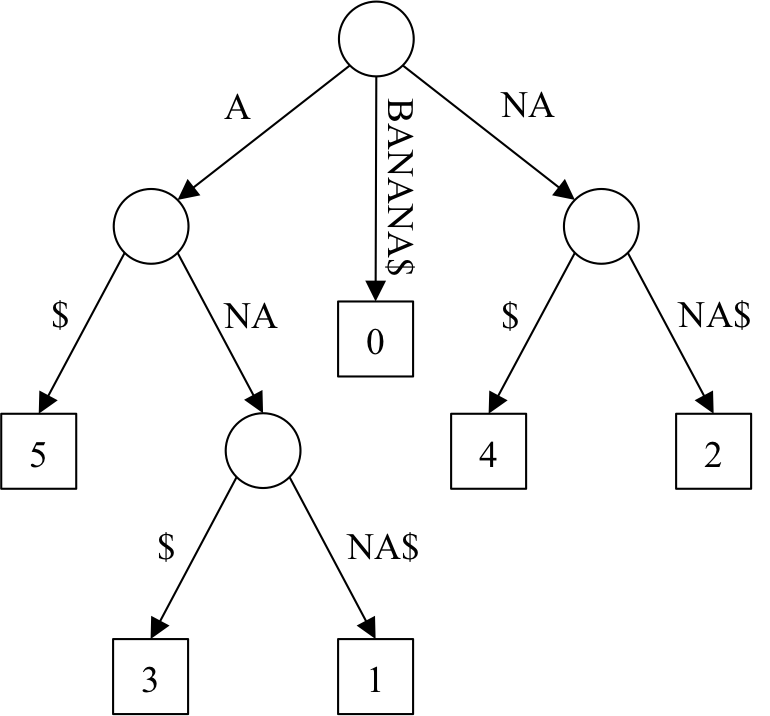
\includegraphics[height = 2in]{figures/banana.png}}
\fbox{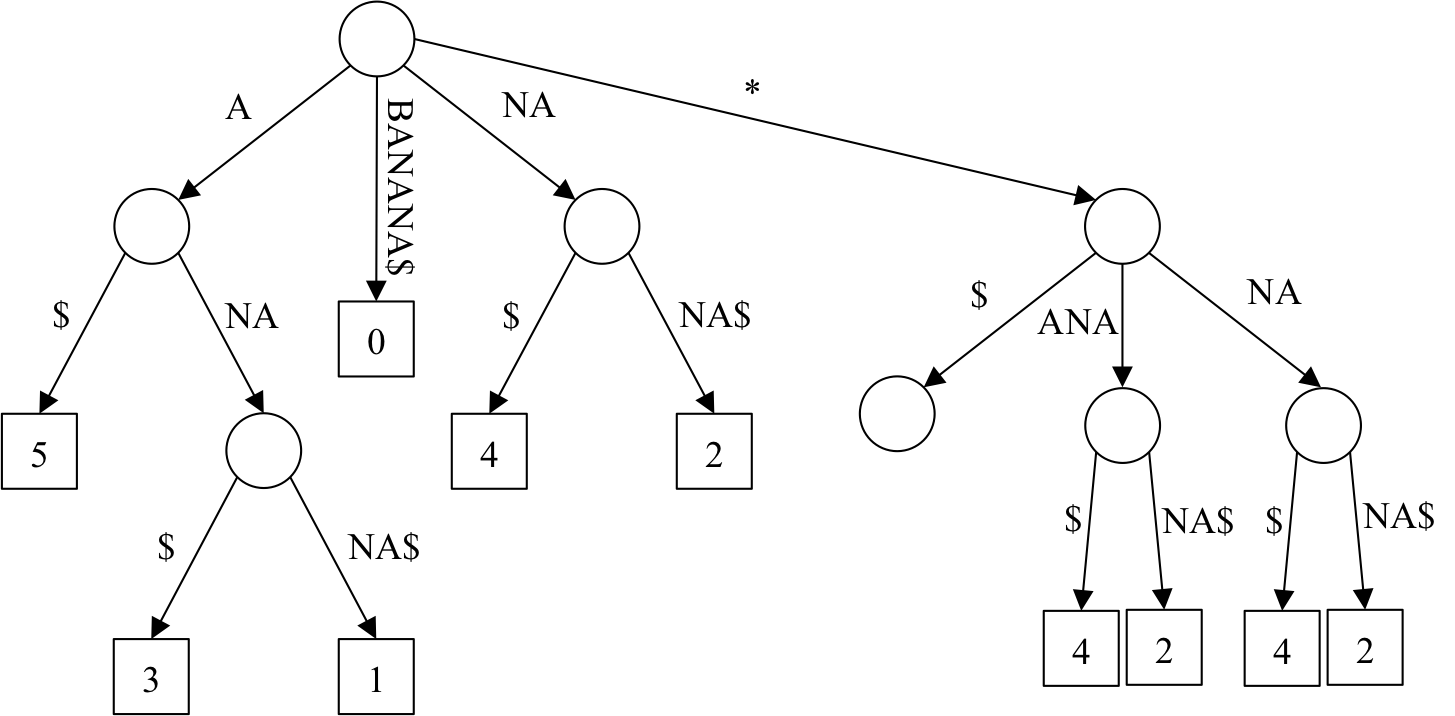
\includegraphics[height = 2in]{figures/bigspace.png}}
\end{center}
\label{fig:sample}
\caption{\small{On the left is the standard suffix tree for $t =$ BANANA. On the right, the suffix tree has been modified to contain a wildcard subtree at the root. Note that the big space, fast query solution discussed in Section 1.4 requires wildcard subtrees be created between every letter.}}
\end{figure*}

\subsection{Cole et al. Solution 1: Centroid Path Decomposition with Slow Query}

In 2004, Cole et al. provided a solution to this problem which achieves faster query time that the first solution, but less space than the second solution. In order to achieve this, the suffix tree is first decomposed into \textit{centroid paths}. The centroid path from the root to one of its descendant leaves is the path which follows the edges with the most descendant leaves (breaking ties arbitrarily). For nodes hanging off of this centroid path, centroid paths are created recursively. The centroid edge of a node is the outgoing edge of the node which lies along a centroid path. By construction, each node has exactly one centroid edge. Figure 1.2 shows the centroid path decomposition of an example suffix tree.

Like the big space solution described above, the Centroid Path Decomposition (CPD) solution builds wildcard subtrees. However, the wildcard subtrees only include suffixes below the node which do not lie along the centroid edge of that node. With this construction, the space to store the suffix tree is only $O(t\log^k{t})$.

The general idea for the query is that whenever we reach a wildcard, we have to explore both the edge along the centroid path and the wildcard edge. Formally, to perform a query, we begin by dividing the query $p = p_0*p_1*\hdots*p_k$, where each of the segments $p_i$ contain no wildcards. We begin by performing the following steps for $i = 0$, and continue until we have either finished with $i = k$ or have discovered a place where $p$ diverges from $t$.

\begin{enumerate}
\item Perform a standard query for $p_i$. Say that this query ends at position $v$ in the tree (which could be a node or along an edge).
\item If $v$ has depth equal to the length of $p_i$ below the starting point, then the query continues. Otherwise $p_i$ must diverge from $t$ and we return no matches.
\item If $v$ is a node:
\begin{enumerate}
\item Advance once character along the centroid path (to account for the wildcard), and then recurse from that location on $p_{i + 1}$.
\item Recurse from the root of the wildcard subtree rooted at $v$ on $p_{i + 1}$.
\end{enumerate}
\item Otherwise $v$ is a point along an edge. Advance one character along the edge and then recurse from that location on $p_{i + 1}$.
\end{enumerate}

If the query returned locations within the tree, we report all the leaf descendants of those locations as matches. For each wildcard, we might branch and explore two different edges. Thus, the total time for this query is $O(2^kp)$.

\begin{figure*}[!t]
\begin{center}
\fbox{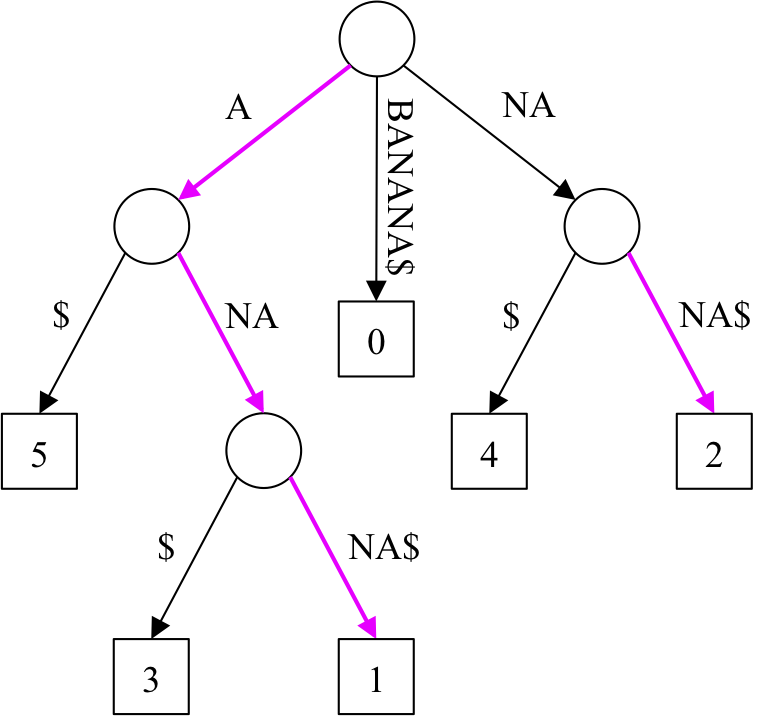
\includegraphics[height = 2in]{figures/centroid.png}}
\fbox{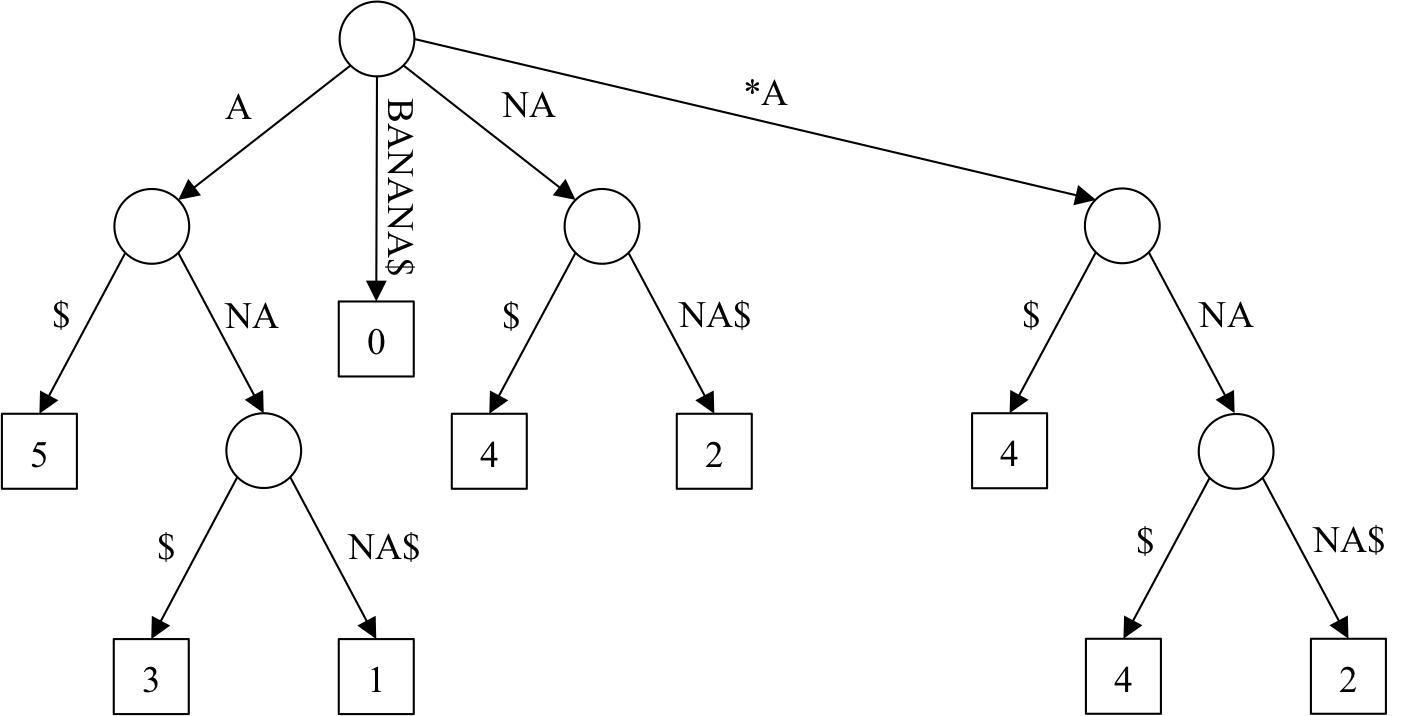
\includegraphics[height = 2in]{figures/wildcardcentroid.png}}
\end{center}
\label{fig:sample}
\caption{\small{On the left is the standard suffix tree for $t =$ BANANA. On the right, the suffix tree has been modified to contain a wildcard subtree at the root. Note that the big space, fast query solution requires wildcard subtrees be created between every letter.}}
\end{figure*}

\subsection{Cole et al. Solution 2: Centroid Path Decomposition with Fast Query}

In their paper, Cole et. al suggested a way to speed up the query time by using a carefully constructed longest common prefix (LCP) query instead of walking down the tree as we did in Step (1) above. The structure is the same as that described in the previous section. We will need to augment the tree with additional information, but we will be sure that the information never takes more than linear space in the size of the tree. Thus the space is still $O(t\log^k{t})$.

This new algorithms calls for preprocessing of $p$ which takes time $O(p)$. The LCP query takes time $O(\log\log{t})$. When we replace Step (1) from above with this LCP query, executing the entire query will take time $O(2^k \log\log{t})$. Thus, the overall time of the query will be $O(p + 2^k\log{\log{t}})$.

Let $S$ be the original suffix tree on $t$. In order to be able to answer LCP queries, we need to build some structures into our suffix tree. We will refer to these structures collectively as the LCP structure. An LCP structure needs to be built for each subtree hanging off a centroid path. All LCP structures are built as part of the preprocessing of the text.

Next we describe the LCP query. Formally, the LCP query takes a node $r$ and query text $p_i$ (with no wildcards), and returns the location $v$ which corresponds to the deepest location at which $p_i$ could be matched, starting at $r$. For now, we will assume that the subtree rooted at $r$ contains its own LCP structure. Because we don't build an LCP structure on every subtree, this may not actually be the case. After we describe the query, we will describe how to handle the case where $r$ is not at the root of some LCP structure.


Let $T$ be an arbitrary subtree on which we are building the LCP structure. First, the LCP structure on $T$ needs to be able to return the LCA (least common ancestor) of any two nodes in $T$. This can be done in space $O(|T|)$ with constant time queries using the techniques described in \cite{lec}.

Next, the LCP structure needs to support weighted level ancestor (WLA) queries. Given a node $v$ and a height $h$, a WLA query should return the position at height $h$ above $v$ in $T$. The (unweighted) level ancestor problem can be solved in constant time and $O(|T|)$ space \cite{lec}. The same ideas can be used to solve the weighted level ancestor problem, but the query time increases to $O(\log\log{t})$ due to the need to make a predecessor query.

Finally, each leaf in $T$ needs to store the index of its corresponding suffix in lexicographic order in $S$. We will refer to this value as $I_x$, where $l_x$ is some leaf node. Note that we store the index of this suffix in $S$, even though we are currently building a LCP structure on $T$. Then, given the index $I_x$ of a leaf, we need to return the two leaves in $T$ which have indices which are the predecessor and successor of $I_x$. This can be done in $O(\log\log{t})$ by storing the indices of all the leaves of $T$ in a $y$-fast trie.

Recall that we have divided $p$ into $p_0*p_1*\hdots*p_k$. When we receive a query $p$, we perform the following preprocessing for each $p_i$. Our goal is to determine, for each $p_i$, the \textit{index} $g_i$ of $p_i$, and also the leaf with which $p_i$ has the most overlap. We determine this value as follows.

\begin{enumerate}
\item Proceed like a standard query in $S$ for $p_i$, noting the endpoint.
\item Compute the leaf $l_i$ corresponding to the closest string to $p_i$, lexicographically. This can be found easily as long as each node has a pointer to its leftmost and rightmost leaf descendants. Also store $h_i$, the length of the longest common prefix of the suffix on $l_i$ and $p_i$.
\item If the suffix at $l_i$ comes before $p_i$ lexicographically, $g_i = I_i + \frac{1}{2}$. Otherwise $g_i = I_i - \frac{1}{2}$.
\end{enumerate}

It takes $O(p_i)$ to perform the preprocessing for any given $p_i$, so the total time to perform the preprocessing is $O(p)$. Once we have completed the preprocessing, then we are prepared to complete an LCP query. The query is computed as described below.

\begin{enumerate}
 \item Look up the leaves in $T$ with lexicographic indices corresponding to the predecessor (call this $l_p$) and successor (call this $l_s$) of $g_i$. Each leaf should also store a pointer to the leaf in $S$ with the same index.
 \item Compute $h_p$, the depth of the node $LCA(l_p, l_i)$ in $S$, and symmetrically $h_s$ from $LCA(l_s, l_i)$.
 \item Compute $\max\{h_p, h_s\}$. Without loss of generality assume the maximum was $h_p$. All further steps are symmetric if $h_s$ is chosen.
 \item Compute $h = \min\{h_i, h_p\}$. The represents the amount of overlap between $p_i$ and $T$.
 \item Let $d_p$ be the depth of the predecessor. Return $WLA(l_p, d_p -h)$.
\end{enumerate}

Steps (1) and (5) take $O(\log\log{t})$ due to the structures described above, and Steps (2), (3), and (4) take constant time. Thus, the overall time to complete this query is $O(\log\log{t})$.

Finally, we need to handle the case where we want to perform an LCP query on a node $r$ which is not at the root of an LCP structure. To perform this query, we will carefully choose a descendant node which is the root of an LCP structure, and then perform the LCP query from there. Let $T$ be the subtree which is rooted at the nearest ancestor of $r$ with a LCP structure. We perform an LCP query on a node not at the root of an LCP structure as follows.

\begin{enumerate}
\item Let $C$ be the centroid path in $T$ which contains $r$ (each node stores a pointer to its centroid path).
\item Find the leaf $l_u$ in $S$ corresponding to the suffix represented by the portion of $C$ below $r$. To do so:
\begin{enumerate}
\item Get the offset in $t$ of the leaf in $T$ at the end of $C$ (each leaf stores this information).
\item The offset of $l_u$ in $t$ is equal to this offset plus the depth of $r$ in $T$.
\item Look up the leaf in $S$ corresponding to this offset (we can store a table of these pointers).\end{enumerate}
\item Compute $h'$ as the depth of node $LCA(l_u, l_i)$ in $S$.
\item Let $h = \min\{h_i, h'\}$.
\item Find the position $v$ at height $h$ below $r$ on $C$. To do this, for each centroid path we store a $y$-fast trie containing depths of all the nodes along $C$.
\item If $v$ is not a node, then return position $v$. Otherwise, perform another LCP query on the child of $v$ corresponding to the next letter of $p_i$. This child will be the root of an LCP structure since it is hanging off a centroid path.
\end{enumerate}

Steps (2), (5), and (6) take $O(\log\log{t})$, and steps (1), (3), and (4) can be done in constant time. Thus, we have an overall LCP query time of $O(\log\log{t})$ for any node.

Now we can perform a query by first preprocessing $p$, and then continuing with the steps outlined in Section 1.5, with the modification that instead of performing a standard query in Step(1) we perform an LCP query. The overall time of this algorithm is then $O(p + 2^k \log\log{t})$.



\section{Methodology}


\section{Results}


\section{Discussion}

 \begin{thebibliography}{9}
\bibitem{cole}
Richard Cole, Lee-Ad Gottlieb, and Moshe Lewenstein.
 Dictionary matching and indexing with errors and don't cares.
 In \textit{Proc. 36th ACM Symposium on Theory of Computing (STOC)},
 pages 91--100, 2004.
 
 \bibitem{lec}
 Erik Demaine. Least Common and Level Ancestors. MIT 6.851 Lectures 15 Notes Spring 2014. http://courses.csail.mit.edu/6.851/spring14/lectures/L15.pdf
\end{thebibliography}

\end{document}
